\section{Hauptteil 1}\label{sec:hauptteil1}

\subsection{Beispiel Zitate}\label{subsec:beispielZitate}

Beispiel Zitat Buch: \cite[S. 25-26]{bspBuch2009} und Beispiel Zitat Website: \cite{bspWebsite2014}.


\subsection{Beispiel Querverweise}\label{subsec:beispielQuerverweise}

Beispiel Querverweis 1: (Siehe Kapitel \ref{sec:grundlagen}). \\

Beispiel Querverweis 2: (Siehe Kapitel \ref{subsec:beispielBild}). 


\subsection{Beispiel Bild}\label{subsec:beispielBild}

\begin{figure}[htbp] 
  \centering
     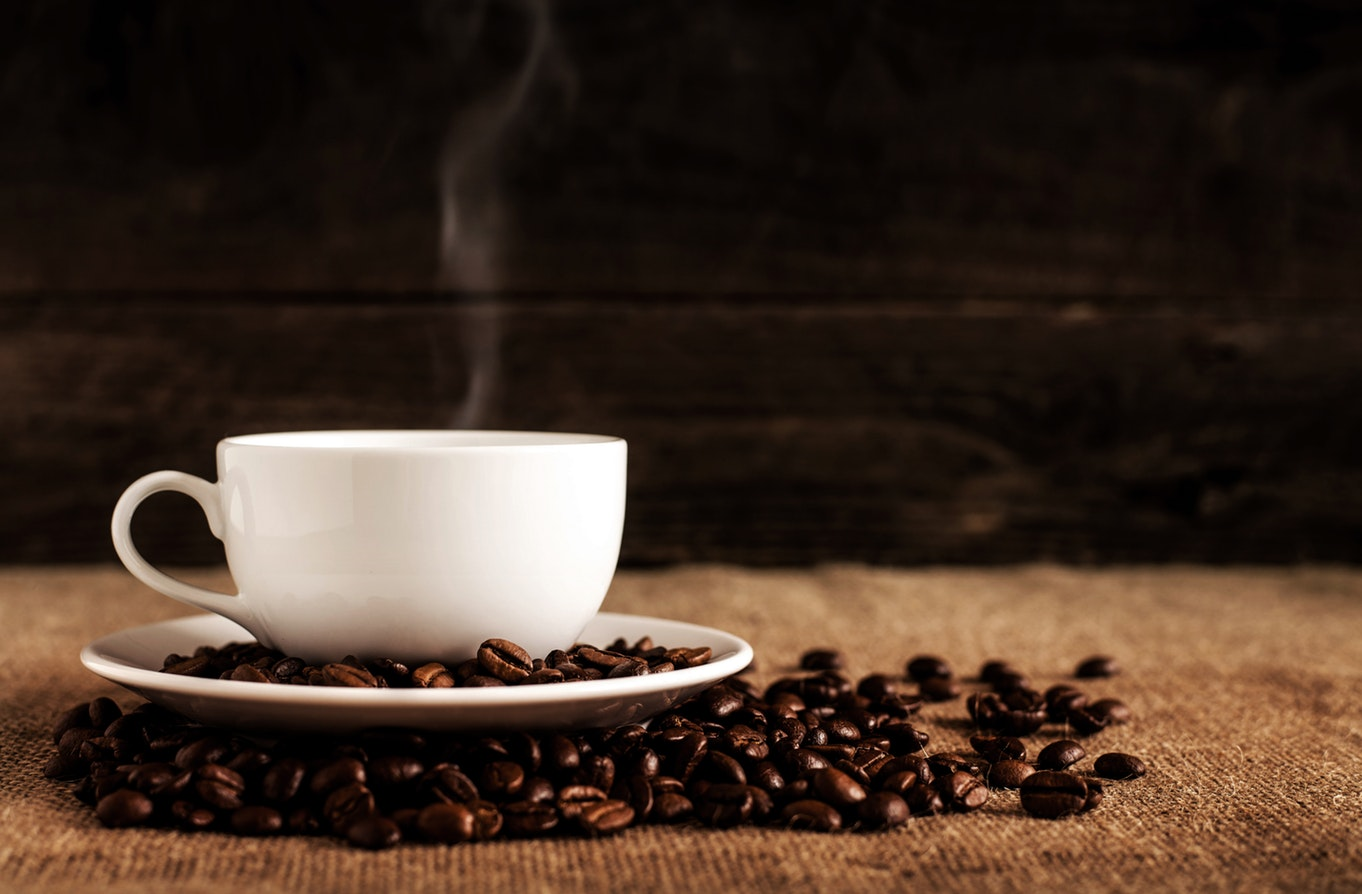
\includegraphics[width=0.7\textwidth]{resources/img/example_picture.jpg}
  \caption{Beispiel Bild}
  \label{fig:Bild1}
\end{figure}


\subsection{Beispiel Abkürzung}\label{subsec:beispielAbkuerzung}

Bei der ersten Verwendung wird die Langform mit der Abkürzung in Klammern ausgegeben: \ac{DIN} \\

Ab dann nurnoch die Kurzform:  \ac{DIN} 